\chapter{Aurelia}
\label{ch:01}



\begin{center}
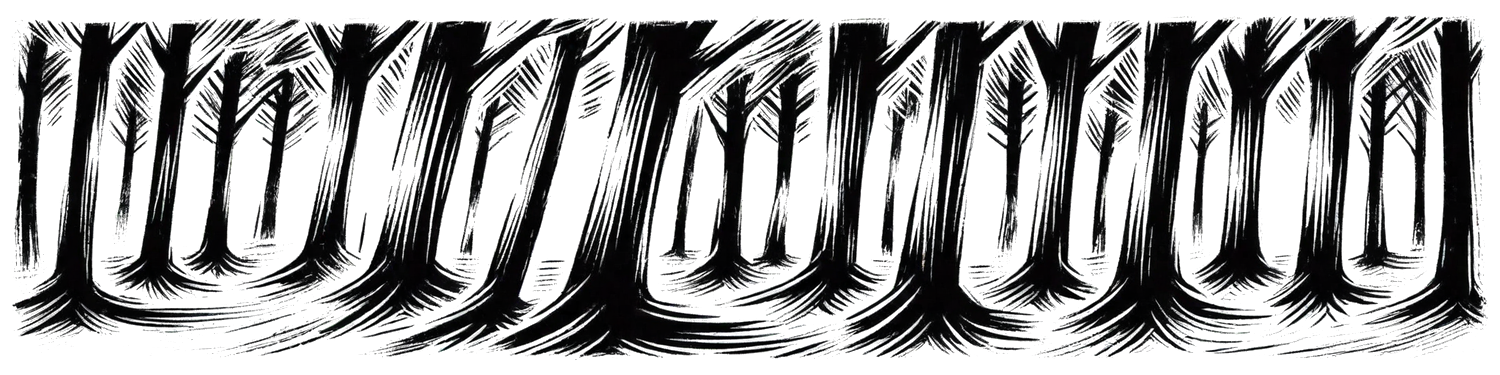
\includegraphics[width=\textwidth]{images/chapterImages/genesis_sketch_00053_.png}
\end{center}

The light came first, threading through the canopy in narrow shafts that turned the mist to silver. She stood in the clearing, perfectly still, her head tilted at an angle that would have seemed awkward if held by another creature but appeared natural on her. The position hadn't changed in three hours.

Her eyes—large, forward-facing, amber in the growing dawn—tracked a point above the treeline. Not the sun. Something else. A star that didn't belong to the familiar patterns, though a human observer wouldn't have known to look for it. Wouldn't have known it was wrong.

She was small for her kind, no taller than a human child, with a body built for precision rather than power. Feathers covered her in layers of gray-brown that caught the morning light like water. Her tail extended behind her, held parallel to the ground, perfectly balanced. Three-clawed hands rested against her sides, the killing claw on each foot tucked up and away from the soft earth.

The mist moved around her. Insects began their morning chorus. Somewhere in the distance, something larger crashed through undergrowth. She didn't react to any of it.

Her breathing was so slow as to be almost imperceptible. Once every forty seconds, her ribcage expanded slightly, contracted. The rest of her remained absolutely motionless. A fern frond brushed against her leg in the breeze. She didn't acknowledge it.

In the canopy above, a small mammal—no bigger than a rat, with large eyes and grasping hands—picked its way along a branch. It paused, looked down at her, seemed to calculate distance and threat. Continued on its path. She wasn't hunting. The mammal understood this somehow, or simply trusted its assessment. It disappeared into the upper leaves.

The star point—if one could call it that, this anomaly in the pre-dawn sky—remained constant. She remained constant. The only movement was the slow turning of the planet beneath her feet, the gradual shift of that point across the sky as the hours passed.

A larger dinosaur emerged at the clearing's edge. Twice her size, heavier, with different feather patterns. It paused when it saw her, head cocking in what might have been curiosity or recognition. It didn't approach. After several seconds, it moved along the clearing's perimeter and vanished back into the forest. She hadn't looked at it.

Four hours now. The sun cleared the trees, burning away the mist. The temperature rose. Still she stood.

An observer might have called it meditation. Might have called it instinct, some deep-seated migratory awareness, a celestial navigation system encoded in her genes. They would have been wrong, but they would have had no way of knowing.

Her pupils contracted in the growing light but never left their focus point. The star was gone now, washed out by daylight, but she knew exactly where it was. She could feel its position in the same way another creature might feel the sun on their face. She knew where it would be tonight. Tomorrow night. A thousand nights from now.

Behind her eyes, something vast and intricate turned. Calculations that would have taken a human mathematician days with pencil and paper unfolded in the space of heartbeats. Trajectories. Velocities. Mass and gravity and the shape of orbits. The numbers built on themselves, layer upon layer, until they formed something like certainty.

But to an observer, she simply stood. Watching the sky.

Five hours. The heat of midday approached. She didn't seek shade.

A young one—barely past infancy—tumbled into the clearing, chasing something small and buzzing. It saw her and froze, perhaps sensing it had intruded on something important. It watched her watching the sky. After a moment, it mimicked her posture, head tilted up, trying to see what she saw. Finding nothing, it lost interest and bounded away.

She never looked down.

The sun moved. Shadows shortened, then lengthened in new directions. Six hours. Seven.

Finally, as the light began to fail and the first evening insects emerged, she moved.

Not suddenly. There was no startle, no shake to loosen stiff muscles. She simply transitioned from absolute stillness to motion as if the stillness had been the motion all along and this was merely a different expression of it.

She walked to the center of the clearing where the ground was bare earth, packed hard by countless feet over countless seasons. Here she stopped.

For a moment she was still again, but differently. Not the stillness of observation. The stillness of decision.

Then she began to arrange stones.

There were three of them, each roughly the size of her clenched hand, scattered at the clearing's edge where water runoff had deposited them seasons or years ago. She picked up the first—not with her hands but with her foot, the killing claw extending to hook it delicately—and carried it to the clearing's center. Set it down with absolute precision.

She stepped back. Looked at it. The angle was wrong by perhaps half a degree. She adjusted it with one clawed toe, the movement so small it barely counted as motion at all.

The second stone went three body lengths away, exactly. She paced it off, each step identical to the last. Set it down. Stepped back. Adjusted. The alignment had to be perfect. It was.

The third stone completed the triangle. The geometry was exact. The angles related to each other in specific ways—not the simple 60-60-60 of an equilateral form, but something more complex. Something that encoded information in its very shape.

She walked around the formation once, examining it from every angle. Made no adjustments. It was correct.

Then she stood in the triangle's center, between the three stones but not touching any of them, and looked up at the darkening sky. The star wasn't visible yet. Soon.

She stayed there until full dark, until the star emerged exactly where she knew it would be. She looked at it for several minutes—not hours this time, just minutes—and something in her posture might have suggested satisfaction, though that was an interpretation an observer would impose. She was simply still. Looking.

Then she left the clearing.

Her movements through the forest were economical, purposeful. She knew this path without needing to see it clearly. She avoided the clearings where others of her kind gathered in the evening. Avoided the water sources where larger creatures drank. She moved through the spaces between, the quiet places.

She didn't look back at the clearing. Didn't need to. The stones were exactly where they needed to be. Tomorrow she would return. Tomorrow she would watch the star again, though its position would have shifted slightly, predictably. Tomorrow she would calculate again, adding new data to the vast architecture of understanding that existed behind her eyes.

The forest at night was loud with life. Calls and cries and the constant rustle of movement. She moved through it like water, touching nothing, disturbing nothing, until she reached the hollow tree where she roosted.

She settled into the space—not a nest, simply a cavity that fit her form—and tucked her head under her arm, the feathers settling into place. Her breathing slowed. The calculations continued even as something like sleep approached, processing the day's observations, integrating them into the larger pattern, the shape of certainty that grew more solid with each passing cycle.

In the clearing, the three stones sat in their perfect geometry. Moonlight touched them. They were just stones. Just arrangements of matter. They meant nothing.

They meant everything.

But there was no one to read them. Not yet. Not for a very long time.

Aurelia slept, and dreamed of trajectories.

